\documentclass[jocse]{jocseart}

\usepackage{booktabs}
\usepackage[utf8]{inputenc}
\usepackage[english]{babel}

% Copyright
\setcopyright{jocsecopyright}
\jocseDOI{10.22369/issn.2153-4136/x/x/x }

\pagestyle{plain}
\pagenumbering{gobble}

\usepackage{cleveref}
\usepackage{todonotes}
\usepackage{graphicx}
\graphicspath{{./fig/}}
\DeclareGraphicsExtensions{.png,.pdf,.jpg,.jpeg}

\newcommand{\jk}[1]{\todo[inline]{JK: #1}}
\newcommand{\ag}[1]{\todo[inline]{Anja: #1}}
\newcommand{\kh}[1]{\todo[inline]{KH: #1}}

\begin{document}
\title{One Year HPC Certification Forum in Retrospective}

\author{Julian Kunkel}
\affiliation{%
  \institution{University of Reading}
  \streetaddress{}
  \city{Reading}
  \state{United Kingdom}
  \postcode{}
}
\email{j.m.kunkel@reading.ac.uk}


\author{Kai Himstedt}
\author{Nathanael Hübbe}
\affiliation{%
  \institution{Universität Hamburg}
  \streetaddress{}
  \city{Hamburg}
  \state{Germany}
  \postcode{}
}

\author{Weronika Filinger}
\affiliation{%
  \institution{EPCC, The University of Edinburgh}
  \streetaddress{}
  \city{Edinburgh}
  \state{United Kingdom}
  \postcode{}
}

\author{Jean-Thomas Acquaviva}
\affiliation{%
  \institution{DDN}
  \streetaddress{}
  \city{Paris}
  \state{France}
  \postcode{}
}


\author{Anja Gerbes}
\affiliation{%
  \institution{Goethe-Universität}
  \streetaddress{}
  \city{Frankfurt am Main}
  \state{Germany}
  \postcode{}
}

\author{Lev Lafayette}
\affiliation{%
  \institution{University of Melbourne}
  \streetaddress{}
  \city{Melburne}
  \state{Australia}
  \postcode{}
}

\renewcommand{\shortauthors}{J. Kunkel et al.}


\begin{abstract}

The ever-changing nature of HPC has always compelled the HPC community to focus a lot of effort into training of new and existing practitioners. Historically, these efforts were tailored
 around a typical group of users possessing, due to their background, a certain set of programming skills. However, as HPC has become more diverse in terms of hardware, software and
 the user background, the traditional training approaches became insufficient in addressing training needs of our community. This increasingly complicated HPC landscape makes
 development and delivery of new training materials challenging. How should we develop training for users, often coming from non-traditionally HPC disciplines, and only interested in
 learning a particular set of skills? How can we satisfy their training needs if we don't really understand what these are? It's clear that HPC centres struggle to identify and overcome the
 gaps in users' knowledge, while users struggle to identify skills required to perform their tasks.

With the HPC Certification Forum we aim to clearly categorise, define, and examine competencies expected from proficient HPC practitioners.
In this article, we report the status and progress this independent body has made during the first year of its existence. The drafted processes and prototypes are expected to mature into a
holistic ecosystem beneficial for all stakeholders in HPC education.
\end{abstract}

%
% The code below should be generated by the tool at
% http://dl.acm.org/ccs.cfm
% Please copy and paste the code instead of the example below.
%
\begin{CCSXML}
\end{CCSXML}



\keywords{}

\maketitle

\section{Introduction}

There is a generally accepted set of skills and competencies necessary to efficiently use HPC resources.
This skill set depends on the role and domain of the practitioner but also on the available infrastructure of the center providing the computing resources.
For example, a scientist needing to run an application on a specific machine may need basic skills in Linux, MPI, environment modules, and knowledge about the batch scheduler, e.g., Slurm.
Now rather than providing that scientists with a list of instructions to be followed in a copy and paste fashion or a never-ending list of things they should know, we want them to understand each of the required steps without having to learner everything about it, but at the same time understand how it fits into the bigger picture of using an HPC system.
For instance, understanding Slurm is a good example of a very fine-grained skill that fits under a more generic skill defined as "resource management", illustrating concepts across the rich variety of available resource managers.

Most institutions operating HPC systems offer regular training events focusing on general aspects of their supercomputer's hardware architecture, software stack, application development environment  and various tuning and debugging tools.
It is understandable why the materials they are geared towards the special demands of the institutions they support and its specific HPC environment.
The problem is that teaching content typically covers only a small part of basic HPC skills necessary to use other HPC systems.
This approach of teaching only specific implementations, tools or workflows, instead of concepts behind them makes a move to a different system or tool unnecessary complicated.
Narrowing the scope of training events make sense from the HPC provider perspective, but is not very conducive to development of more comprehensive learning environment that provides assessment and certifies the newly acquired skills. So although, certificates are used widely in IT industry to verify certain knowledge, until now there was no similar approach for HPC training.
It is, however, clear that a mapping of competences and certification scheme could address some of the challenges stemming from the constantly growing training needs of our community,

This article describes the current status of the certification program initiated by the HPC Certification Forum.
Our previous work provided a brief overview of the evolution from the project that sparked the HPC Certification Forum \cite{TAHCPKHHSS19} while this article provides details on adopted mechanisms and design decisions.

The article is structured as follows:
First, in \Cref{sec:forum} we introduce the HPC Certification Forum and the certification program.
Then, an overview of the status is given in \Cref{sec:status}, followed by the organisation of competencies discussed in \Cref{sec:skills}.
This leads to the proposal for the certification process in \Cref{sec:certification}.
In \Cref{sec:ecosystem} the whole learning ecosystem is described.
Related work is presented in \Cref{sec:related}.
Finally, the article is concluded in \Cref{sec:conclusion}.

\section{The HPC Certification Forum}
\label{sec:forum}

The HPC Certification Forum (HPCCF) has the role of a (virtual) central authority to curate and maintain the proposed certification program.
The program consists of three parts: the tree of defined competencies, the examination of practitioners to prove they posses those skills, and finally the certification demonstrating their knowledge.
Although, the forum is not involved in development of any training materials or tools, it supports the ecosystem around the competencies.

The HPCCF aims to support existing activities and complements them by providing a unified and clear way of mapping out the relevant HPC competencies.
Thus, the HPCCF does not regulate the content of training material; we purposely separate the definition of skills, the examination and the certification from content delivery.
Similarly, the program does not prescribe a curriculum or any fixed order by which skills need to be obtained. It eases the navigation between different competencies without being overly restrictive.

The forum is organised around a Webpage\footnote{http://hpc-certification.org},  a GitHub repository\footnote{https://github.com/HPC-certification-forum},  and a could-based team collaboration tool (Slack) for communication and monthly meetings.
The membership is divined into three categories: associate, full and steering board.
Anyone can become an associate member free of charge, allowing a passive involvement -- e.g., observing the status, being listed on the webpage.
Full members must actively contribute to the program and have voting rights for the roles of the steering board.
The steering board directs the overall activities and is organised in different responsibilities, i.e., into topic-specific chairs. At the moment the steering board has 9 members.


\section{Overview of the HPCCF activities}
\label{sec:status}

The first year of the HPCCF forum was rich in discussions, both internally and with external partners, resulting in a number of processes and prototype tools being put in place. These are described briefly below, and in more details in the subsequent sections.

\paragraph{Management}
The first steering board has been elected at ISC-HPC 2018.
We established communication channels via webpage, email and Slack for regular discussion.
Slack is also used to conduct our monthly open meetings between members and the steering board.
At beginning video conferencing tools have been used, but the geographical diversity of the attendees influenced the decision to move towards chat-based tools. 
The asynchronous nature and automatic message retention proved to be more productive, and provided a more open and inclusive platform for discussion.    
Meeting notes with action items are extracted from Slack and documented using Google Doc (an online word processor allowing a real-time and multiple-user collaboration).  

The ongoing conversation with various stakeholders involved in HPC education and training, keeps producing more engagement in the forum's activities.   
The member's contributions are voluntarily and follow the schedule agreed between the contributor and the HPCCF board.
The prospective contributions are managed in Trello (a web-based list-making collaborative application), in which each member can manage their own card.

\paragraph{Technical tasks}
The tasks we set out to accomplish are:  1) the definition of competencies; 2) the examination of practitioners;  3) the creation of certificates; and 4) the reinforcement of an ecosystem of tools supporting them.

For all these sub-goals we made substantial progress.
While the definition and organisation of competencies was the main focus, we prototyped various tools and processes that embed the competencies into the wider education ecosystem.

Firstly, considering the pedagogic literature from higher education we finalised the templates for the skills description. 
The effort to map out all of the relevant competencies is still on-going, but the feedback received during a number of events organised by the HPCCF and other members of the HPC education community resulted in the addition of new topics to the first version of the certification program. 

The definitions of the competencies are version controlled with Git, and are publicly available in XML and Markdown format.
A Wiki\footnote{https://www.hpc-certification.org/wiki/} is being used to edit the skills' descriptions, and a navigable and widely customisable JavaScript\footnote{https://www.hpc-certification.org/skills/map/} makes the skill tree easily accessible to the forum members and the end-users alike.

Preliminary processes and tools have been developed and deployed for curation of the examination questions and for conducting an online multiple-choice examination.

\section{Skills}
\label{sec:skills}

A skill is defined as a set of learning outcomes and relevant metadata. 
Within a single skill, there can also be multiple levels (basic, intermediate and expert level) building upon each other and further distinguishing the expertise. 
We expect the practitioners to acquire the lower levels before progressing to more complex levels.

This model can be compared to the classification of school knowledge, for example, a skill with the name “basic arithmetic operations” would include the math skills of addition (being able to add numbers), subtraction (being able to subtract numbers), multiplication (being able to multiply numbers) and division (being able to divide numbers). Operating on two numbers would be a basic level of the skill, whereas mentally operating on hundreds of numbers would be an expert level. Another example could be a skill called "technical drawing", in which being able to draw simple geometric figures would be counted as a basic level, and an ability to draw a complicated mechanical objects would be an expert level. 

The basic level should cover the most relevant aspect of the skill (needed by anyone that uses the skill), whereas the intermediate (used for common exceptional cases) and expert levels (used in special circumstances)  are needed only for a subset of users.
Typically, an institution has only few experts, if any at all.

The skills are organised in a tree structure from a coarse-grained to a fine-grained representation, allowing users to browse the skill based on the semantics.
The root level of our current skill tree is shown in \Cref{fig:skill-tree}. The goal is to finalise the tree this year.
The basic idea is that the skills from the root level simplify the navigation by providing an indication about their scope, e.g., core knowledge, usage of HPC environments, or about programming.
This should allow the user to rapidly drill into the skill representation.
The closer a skill is to the root, the more abstractly it is defined, while leaf nodes cover the knowledge for a specific skill.

As the tree serves the purpose of organising the skills, the references from one branch to a skill in another branch are allowed.
This import feature makes the reuse of the skill definitions possible, at the same time allowing users to navigate the tree according to the semantics.

\begin{figure*}[tb!]
	\centering
	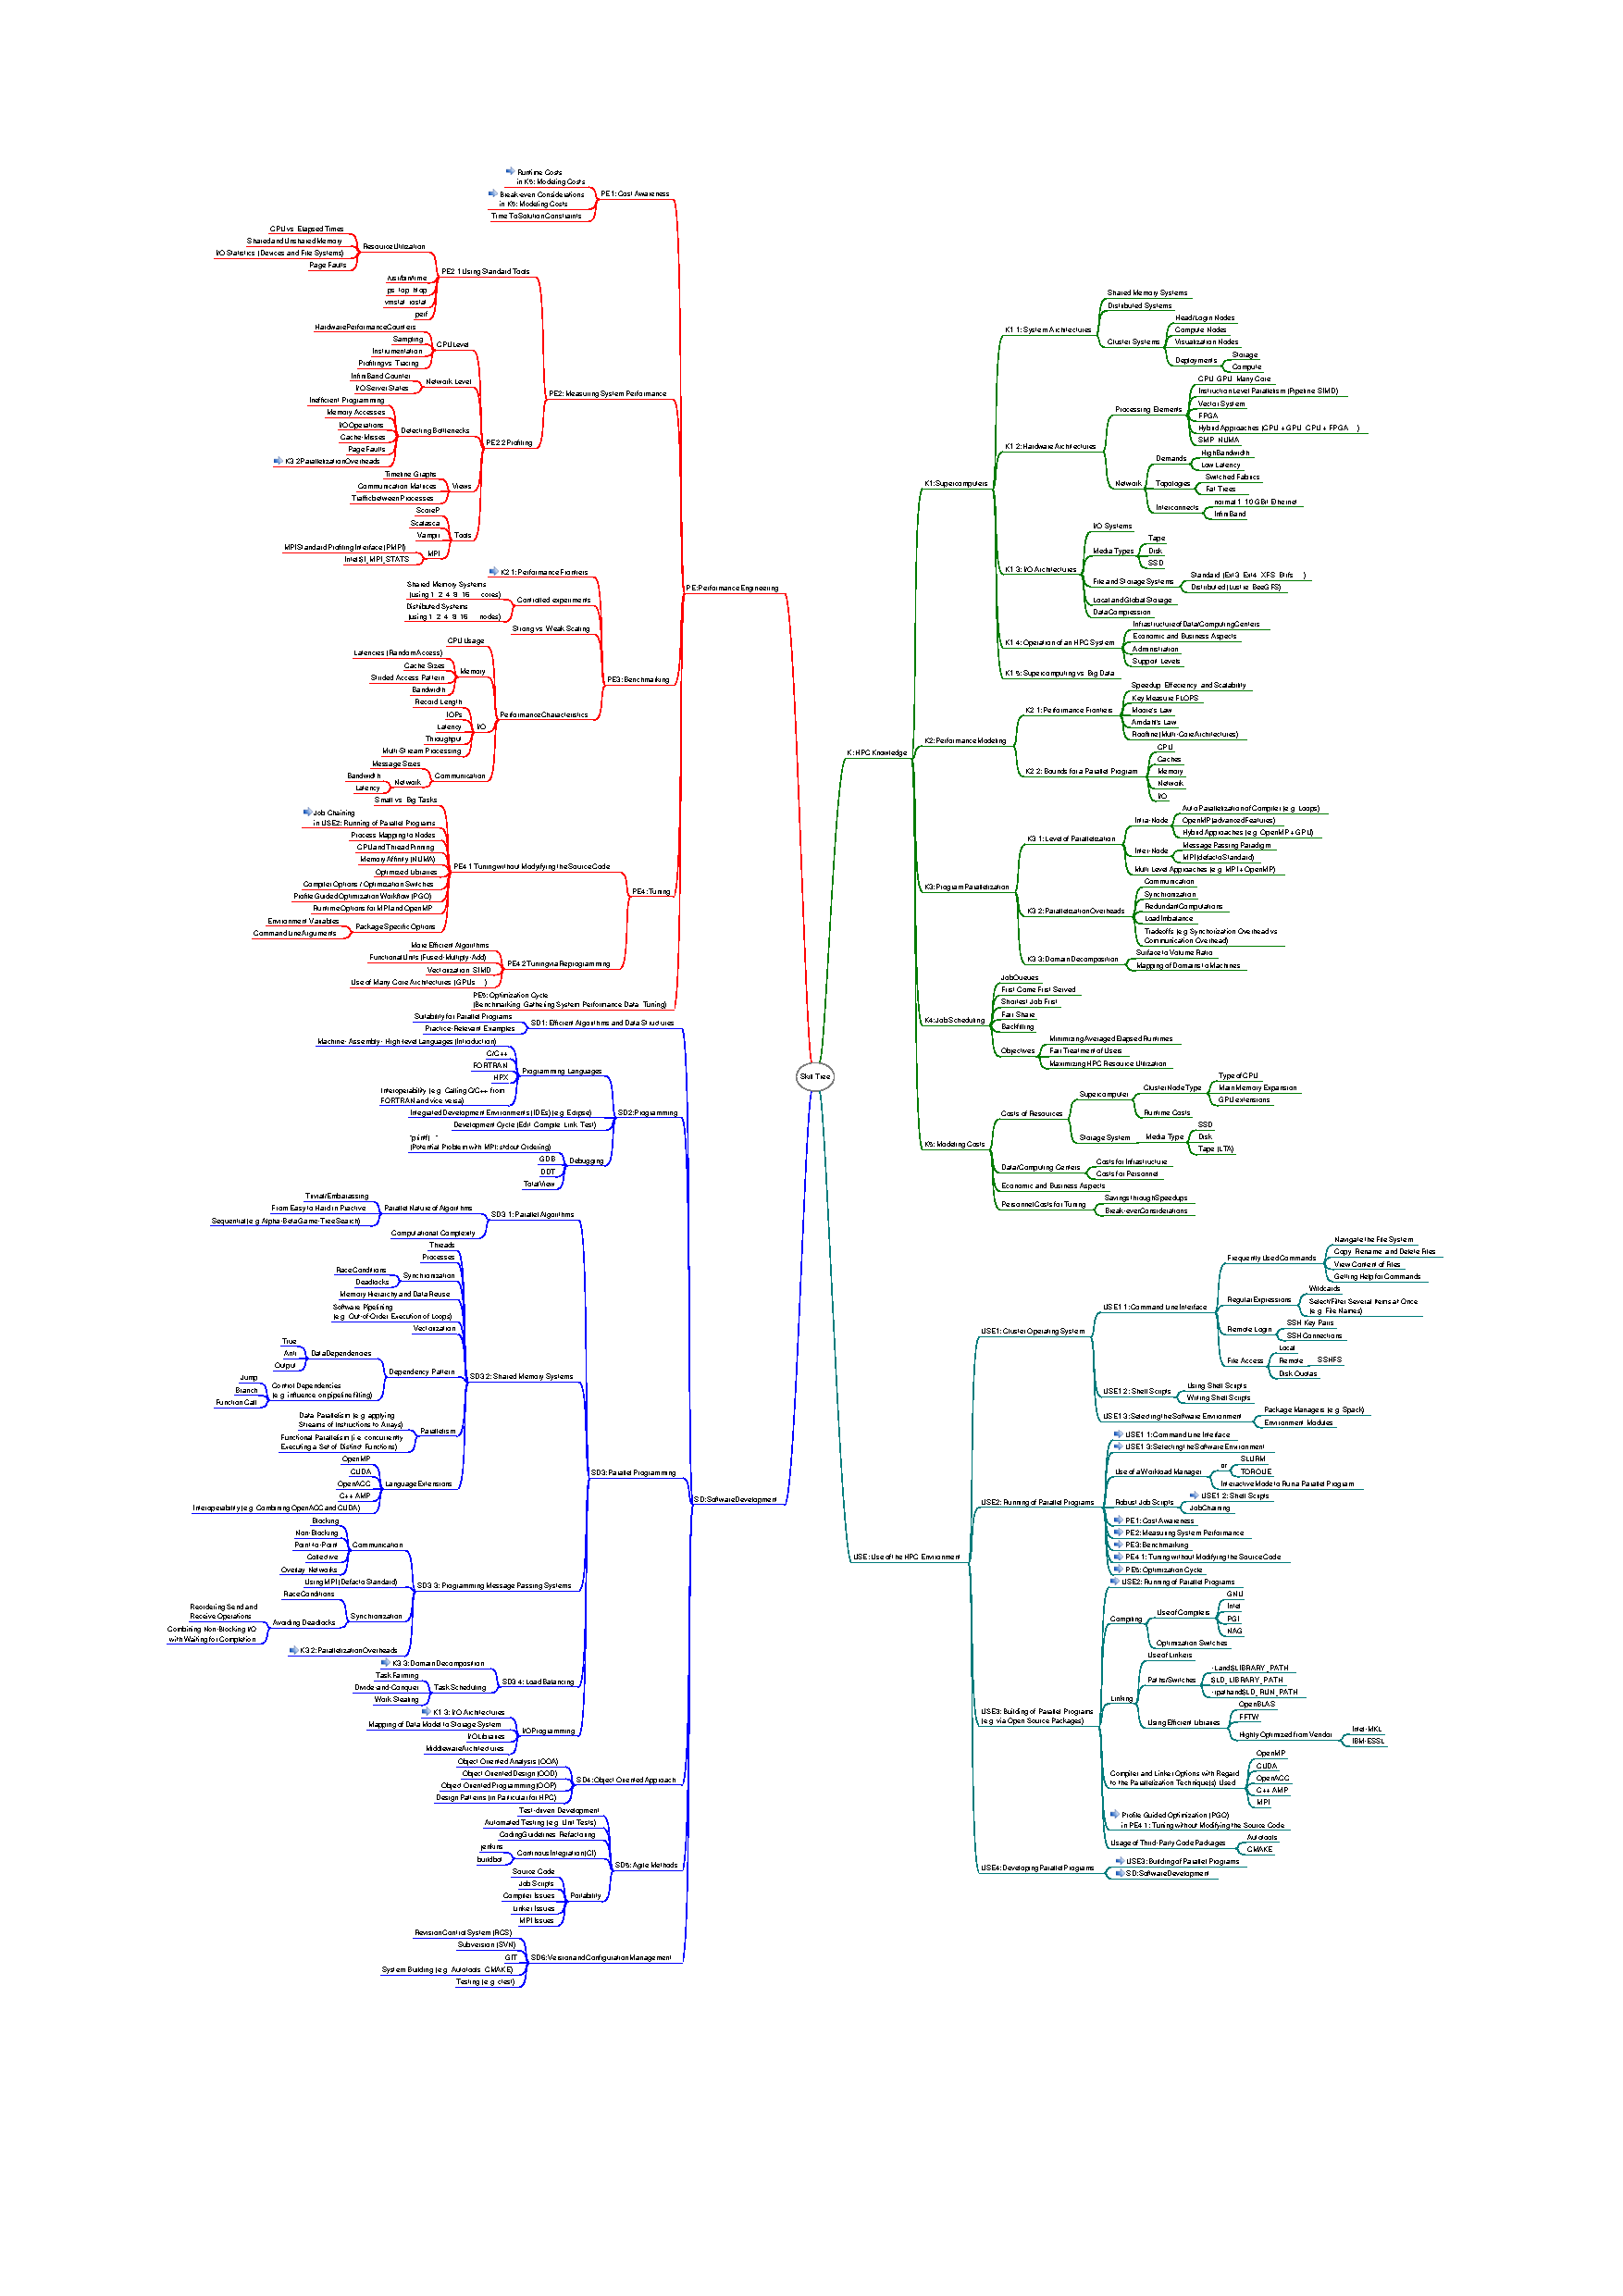
\includegraphics[width=15.0cm]{skill-tree}
	\caption{Skill tree: top level competencies with the PE4 branch expanded.}
	\label{fig:skill-tree}
\end{figure*}

\subsection{Description of a skill}

Each skill on the tree, including the inner nodes, is described in more detail as follows:

\begin{itemize}
  \item \textbf{ID}: ID according to its position in the skill tree. The last character indicates the level of the skill (Basic, Intermediate, or Advanced).
  \item \textbf{Name}: A name capturing the essence of the skill.  
  \item \textbf{Background}: Provides brief information motivating the need for the skill and how it fits into the bigger picture with other skills. 
  \item \textbf{Aims}\footnote{The definition of aims and outcomes follows literature for higher education \cite{williamson2011good} and \url{https://www.heacademy.ac.uk/system/files/assessment-learning-outcomes.pdf}.}: 
  Describe the purpose of the skills, but doesn't really include a list of what a practitioner will learn or do. Explaining what a skill is trying to achieve is not the same as saying how it should be done.  
  \item \textbf{Learning outcomes (LOs)}: Defines briefly what practitioners will learn.
  The objectives are statements what prospective learners are able to do. They should clearly describe or define an action bringing about a measurable/quantifiable increase in understanding of that skill.  
 \end{itemize}

On the leaf level, a skill is fine-grained and orthogonal to other skills -- their narrowed scope means they can be taught in sessions ranging from a 1.5 hour lecture up to a 4 hour workshop.
We believe this granularity allows practitioners to cherry-pick the skills relevant to their circumstances, and lecturers and examiners to prepare small lectures with well-defined content.
For technology-dependent skills on the leaf level (e.g., a specific file system or workload manager) the introductory skills are often provided, as they contribute to the foundation of many specialised skills representing a specific hardware or software technology.

The aggregation within the tree is similar to that found in the education circles. Hussey et al.\cite{hussey2008learning} categorised the aggregation of skills into the following levels: individual teaching events, specified for modules or short courses, and those specified for whole degree programmes. 
Although, Hussey et al. conclude that LOs on the coarse grained level are not useful for high-level education, using a similar concept with relaxed level of granularity/abstraction of the learning outcome fits well within the framework of the certification program.  
\kh{den Satz habe ich nicht genau verstanden; als Leser würde ich mir die Kurzbegründung wünschen, die Hussey et al. für ihre Feststellung anführen}

\subsection{Skill Examples}

This subsection presents an example of an inner-node skill called "Executing parallel applications", as well as its two leaf skills - "Workload manager introduction" and "Slurm workload manager".

\begin{itemize}
  \item \textbf{ID}: USE4.2-B
  \item \textbf{Name}: Executing parallel applications
  \item \textbf{Background}:
  Parallel computers are operated differently than a normal PC -- all users share the system. To ensure a fair and efficient use of shared resources, various operative procedures are put in place. Users must understand these concepts and procedures to be able to run a parallel application on the resources available to them. Moreover, different HPC systems adopt different solution to manage their resources.  
  \item \textbf{Aim}: To enable practitioners to comprehend the concepts and procedures for running parallel applications in HPC environments; to run and monitor the execution of parallel applications on HPC systems.

  \item \textbf{Learning outcomes}:
    \begin{itemize}
    \item explain the concepts and procedures related to resource allocation and job execution in an HPC environment;
    \item run interactive jobs and batch jobs;
    \item understand and describe the content and expected behaviour of job scripts;
    \item change provided job scripts and embed them into shell scripts to run a variety of parallel applications;
    \item analyse the output generated from a job scheduler and understand the cause of typically generated errors.
    \end{itemize}
\end{itemize}

\ag{When I was reading the "learning outcome" of USE4.2B, another category came to mind:
How to write job scripts? How to batch use?
So why not create a case where the learning outcomes overlap?
Since you did the skill examples with USE4.2 in 4.2, I would not do "Figure 1" with extension of PE4 but USE4.
Then you can always look there.
}

The next leaf-level skill describes how workload management works in general, regardless of the specific software implementing it. 
The aim and outcomes defined by the parent skill (described above) are expected to be covered (to a certain extend) and refined by this leaf skill.

\begin{itemize}
  \item \textbf{ID}: USE4.2.1-B
  \item \textbf{Name}: Workload manager introduction
  \item \textbf{Background}: There is a wide range of different workload managers in use. This skill on a conceptual level explains how to use them.
  \item \textbf{Aim}: To enable practitioners to comprehend and describe the basic architecture and concepts of resource allocation on an HPC system.
  \item \textbf{Learning outcomes}:

  \begin{itemize}
  \item comprehend the exclusive and shared usage model in HPC;
  \item differentiate between the batch and interactive job submission;
  \item comprehend the generic concepts and structure of resource manager, scheduler, job and job script;
  \item explain the role of environment variables as a mean to communicate certain settings of your job;  
  \item comprehend job budgeting and accounting principles;
  \item explain the generic steps required run and monitor a single job.
  \end{itemize}
\end{itemize}


The following skill describes a leaf-level skill for the usage of Slurm at the basic level.
While there is no formal dependency to the introduction (skill USE4.2.2-B), it is expected that practitioners have obtained the other skill before learning this one.

\begin{itemize}
  \item \textbf{ID}: USE4.2.2-B
  \item \textbf{Name}: Slurm Workload manager
  \item \textbf{Background}: Slurm is a widely used open-source workload manager, which also provides various advanced features. % \kh{Vorschlag: einige der Highlights anführen: "... , like ..."}. Good idea, but later!
  \item \textbf{Aims}:
  \begin{itemize}
    \item To enable practitioners to use relevant tools to run and monitor parallel applications using Slurm.
    \item To enable practitioners to comprehend and describe the basic structure of Slurm and the related suite of tools.
  \end{itemize}
  \item \textbf{Learning outcomes}:
  \begin{itemize}
  \item run interactive jobs with \textit{salloc}, a batch job with \textit{sbatch};
  \item explain the architecture of Slurm, i.e., the role of \textit{Slurmd}, \textit{srun} and the injection of environment variables;
  \item explain the function of the tools: \textit{sacct}, \textit{sbatch}, \textit{salloc}, \textit{srun}, \textit{scancel}, \textit{squeue} and \textit{sinfo};
  \item explain time limits and the benefit of a backfill scheduler;
  \item comprehend that environment variables are set when running a job;
  \item comprehend and describe the expected behaviour of a simple job script;
  \item comprehend how variables are prioritised when using command line and a script;
  \item change a provided job template and embed them into shell scripts to run a variety of parallel applications;
  \item analyse the output generated from submitting to the job scheduler and typically generated errors.
  \end{itemize}
\end{itemize}

\ag{I could put my slide set online and show the skill tree for the slide set. An example could be shown, there the content described in a skill tree are also explained in slide sets.
Everything under USE 4.2.2 B, I have explained it in my slide set under "Slurm Usage on Goethe HLR cluster".
\\
What I have found and would like to try it out:  http://xlong88.github.io/draw-binary-tree-latex/
Create recursive and automatically a Binary Tree with Tikz and Tikz-qtree.
If we can do it generically then I will be one step ahead with my skill tree for the slide set.
}

The learning outcomes of this skill, marked with B to indicate its basic level, are focusing on the most fundamental knowledge required to use Slurm effectively.
An intermediate version of the skill could, for example, cover how to create reservations or special queues.  

%\begin{itemize}
%  \item \textbf{ID}:
%  \item \textbf{Name}:
%  \item \textbf{Background}:
%  \item \textbf{Aim}:
%  \item \textbf{Learning outcomes}:
%\end{itemize}


\section{Certification}
\label{sec:certification}

A certificate shall serve as a confirmation that a user obtain the expertise in the relevant skills.
Special considerations needs to be given to the certification integrity.  
We must ensure that the learning outcomes of the covered skills are examined to a satisfactory degree, and prevent self-cheating or dishonesty.
Students can always cheat during an examination -- the susceptibility to cheating depends on many factors, including but not limited to the type of exam, methods used for assessment, motivation for taking it,  consequences of failing or scoring poorly, and the possibility and frequency of resits. 

We want to enable a cost-effective assessment (free for the practitioner), so we chose an online examination.
This increases the opportunity for cheating \cite{rowe2004cheating} but we plan to deploy a several strategies to minimise the risk of cheating, such as raising the awareness of the examinees, using a pool of questions, time limits for each question and a delay between registering for and taking the examination. 

Since knowledge can age, each certificate needs to indicated when (month and year) the qualifying examination took place.
Also, because the examination of a single fine-grained leaf-level skill would be too easy for short-term memorisation and more prone to self-cheating, the certificates bundle multiple skills together.
We believe the incentive to deliberately fake the assessment, e.g., by having the exam filled by someone else, and thus, being awarded a certificate, is low.
Therefore, we address this issue in a lightweight fashion only.

A process has also been created for prospective contributors of the examination questions.
The questions are the only proprietary component for the HPCCF -- using restrictive license terms for authors while giving them credit. 
This is considered necessary to minimise the overhead of managing the database containing solutions to the examination questions. 

In the next section, we discuss the process proposed for conducting the examination.

\subsection{Examination Process}

The examination process can be started at any time but a delay is employed before the examination actually starts.
Firstly, a user has to register using their name, email address and optionally an affiliation.
This process is explained, together with privacy policies, on the examination website. 
Next, they need to read a paragraph on the integrity policy defining cheating and encouraging honesty.
Practitioners are asked to opt-in for the policy statement.
Upon receiving this registration, we generate an encrypted token on the server that is returned to the user by email.
At this stage, we do not store any information about the user on the server.

The email contains a link that will start the examination, and the user chooses to start the examination by clicking on it. Only then, the information about the user and the examination start time is stored in a temporary database.

The summative assessment itself is conducted using multiple choice questions. 
Therefore, for each skill, we will develop a pool of questions and answers, and accept external contributions.
Each question has a pool of possible answers (e.g., 10). An examination consists of randomly selected questions with five of their answers, and the practitioner has to decide if each statement is true or false.

Once the user submits the completed exam, all selected answers are stored on the server for validation -- which currently is done manually.
If the user meets the pass criteria (typically 70\% of correct answers) the earned certificate is issued and sent to the user by email.
All personal information about the user is then deleted from the server, but the affiliation and raw responses are preserved.
The affiliation is used for promotional purposes, while the raw responses will be analysed to optimise the questions.
For example, if we identify that most users make the same mistake it may be an indication that either that question or its answer is too ambiguous and should be improved.

If the user didn't meet the pass criteria, they will be informed about their score.
The user can then retry to obtain the certificate after a cool-down period (typically one week), but not immediately afterwards to prevent success via brute force methods.
To enforce this, the information about when the exam was undertaken is linked to the user's name and email.
As the sole purpose of the multiple choice questions is the examination, the incorrectly answered questions will not revealed. 
We assume that high quality training materials available within the HPC community, and covering the individual skills being part of this certification program, offer constructive feedback and other ways of consolidating the newly acquired knowledge. Therefore, the Forum's only concern is to provide the mechanism of certifying whether the learners posses that knowledge or not. As opposed to pointing out gaps in their understanding.   

 %---> ? \cite{epstein2002immediate}.

\subsection{Certificates}

The examinees that pass the examination are awarded a corresponding certificate. Such certificate consists of two parts: a PDF and a text file. 
The PDF contains the key information making the certificate meaningful. An example of how it may look like is presented in\Cref{fig:awardedCertificate}.
The name and identifier of the certificate is found in the centre, on our example these are "HPC Driving License" and 1, respectively.  
Similar to a driving license, this particular certificate could provide the minimum set of knowledge required to understand and use a typical supercomputer.

The text file a contains the same information, as well as a verification URL that can be given to a third-party to confirm the certificate's credibility. 
It is also PGP signed using the private key of the HPC Certification Forum to allow verification with the public key.


The file looks as follows:
\begin{verbatim}
-----BEGIN PGP SIGNED MESSAGE-----
Hash: SHA512
HPC Certification Forum Certificate
This text confirms that "Julian M. Kunkel" has
successfully obtained the certificate
"HPC driving license" (id: 1) at 02/2019.
Verification URL: https://hpc-certification.org/[...]
-----BEGIN PGP SIGNATURE-----
[...]
-----END PGP SIGNATURE-----
\end{verbatim}

Together both documents should be able to provide enough credibility for the certification to be fully functional within the HPC academic and professional domains. Further improvements will be adopted as required. 

\begin{figure}
  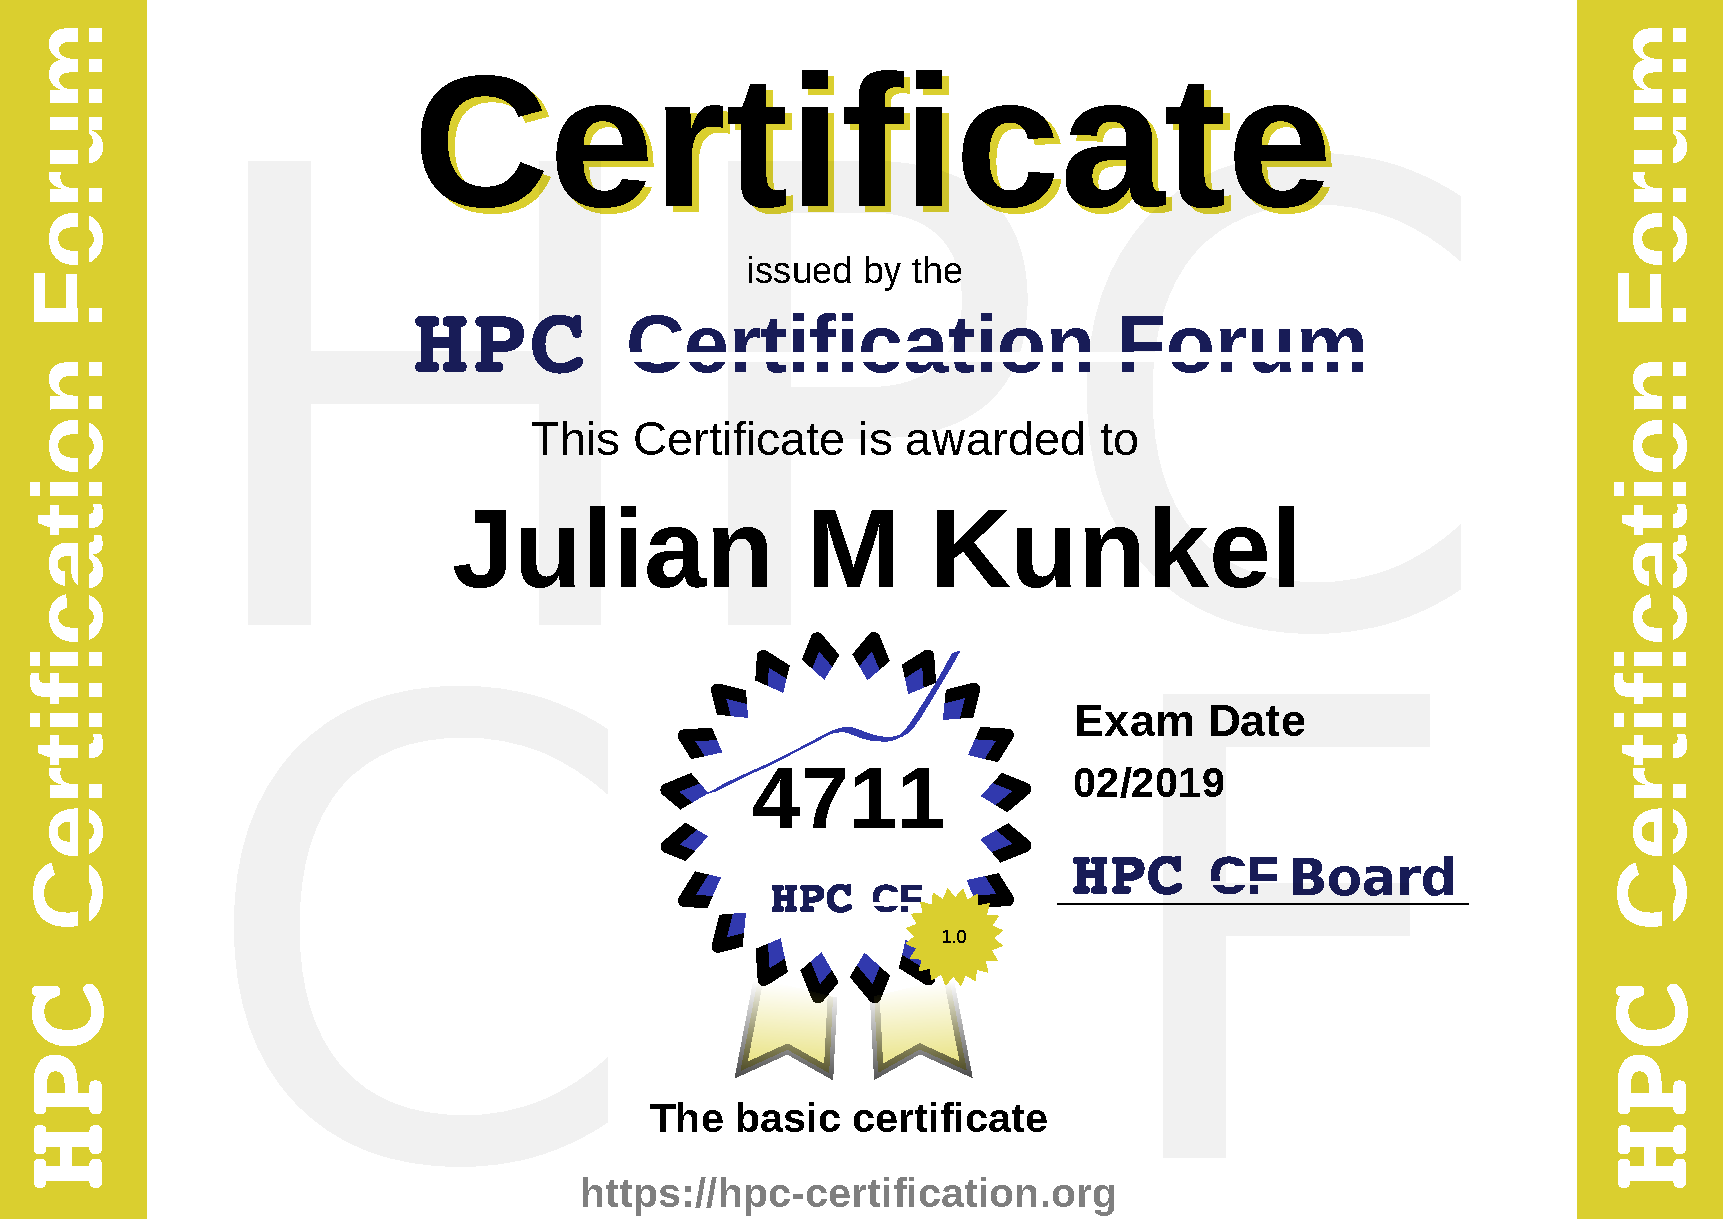
\includegraphics[width=0.48\textwidth]{JulianMKunkel}
  \caption{Draft for an awarded certificate}
  \label{fig:awardedCertificate}
\end{figure}

\section{Ecosystem}
\label{sec:ecosystem}

We encourage the development of an ecosystem around the HPC classification, we are supporting training and tool development.

\subsection{Training Delivery}

The HPC Certification Forum is not developing training material directly or competing with providers of training material.
However, we support individuals and institutions by endorsing and promoting their training materials and courses in two ways.

Firstly, an author of training material is allowed to indicate on the training material itself or on promotional material the fact
which skills are covered by the material completely or partially.
We provide a seal that can be used for that purpose (see \Cref{fig:seal-teaching}).
The reference to the HPCCF and the seal can be used free of charge under the condition that the developer of the training material
registers a link to the material or course on our webpage using an online form. %\footnote{Details of the link will show the email address.}
That way, the HPCCF is informed about the usage of the seal.

Secondly, we will link on our webpage the endorsed training material for the individual skills and certificates.
By using JavaScript and dynamic webpage we will provide various views on the skills with and without links to suitable training materials.

Note that we are not intending to verify the correct usage of the skill explicitly.
However, in case the training material or course doesn't deliver the expected material practitioners may complain and we will remove the training material from our webpage.

We expect that this strategy will lead to the availability of good free training material for most skills while companies and individuals can still charge for effective training courses.
Ultimately, the resulting training material will complement each other leading to a rich variety of content suitable for each individual practitioner, e.g., addressing different learning styles and languages.

\begin{figure}
  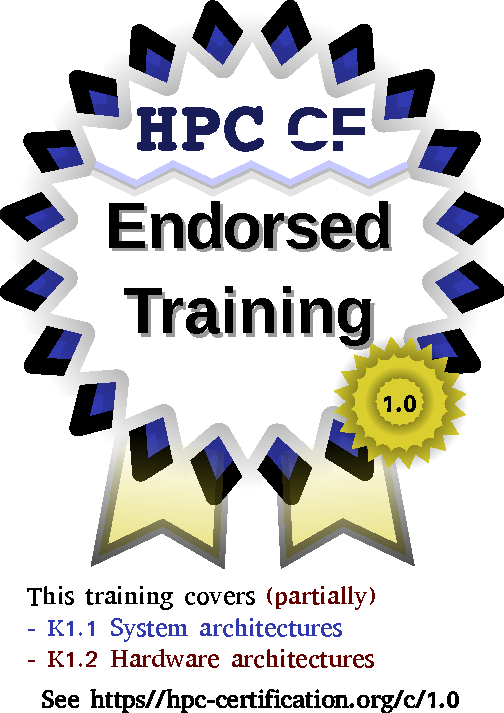
\includegraphics[width=0.3\textwidth]{certified}
  \caption{Draft for the seal for teaching material}
  \label{fig:seal-teaching}
\end{figure}


\subsection{Navigation}\kh{Vorschlag Unterkapitel in "Results" umbenennen oder an anderer Stelle aus "Erwartungsgründen" ein "Results"-Kapitel ergänzen (am besten natürlich auf der Hauptgliederungsebene, aber das wird vermutlich schwierig werden)}
%\paragraph{Navigation}
Thanks to the contributions of the PeCoH project, a JavaScript prototype enables the embedding of a navigable skill tree into a webpage.
The script can be used by different stackholders to present their own view on the skill-tree.
By view we mean the selection and organization of the skills, and the additional information provided when navigating the tree.
For instance, you could have a tree for a specific scientific domain, for a specific data center, or even for the role of the tester of a specific application; it could indicate which skills are mandatory or beneficial for these use cases, providing links to training material or adding further supplementary information.


\section{Related Work}

\label{sec:related}

\jk{Please everyone!}

Relevant work can be classified into approaches to establish a curriculum or the creation of teaching material.
In academia, individual universities offer their own curriculum around scientific computing and HPC, covering theoretical aspects like the software development of numerical applications.
They are not tailored to the needs of a practitioner to actually use HPC systems effectively.
Data centers offer their own material and courses to support their own users.
Several projects address the generation and sharing of teaching material for HPC.
The EuroLab-4-HPC project establishes training in form of (online) courses\footnote{\url{https://www.eurolab4hpc.eu/}}.
The Barcelona Supercomputing Centre (BSC) aims to develop a professional training curriculum \cite{sancho2016bsc}.
The virtual organization XSEDE\footnote{\url{https://portal.xsede.org/web/xup/training/overview}} provides an online system to train the usage of an HPC system, structuring the corresponding information on their website into major topics like “Getting Started”.
The user can navigate the topics and receive further information.

\section{Conclusion}
\label{sec:conclusion}


This allows the re-use of existing content but also allows to create a new ecosystem in which HPC centers or commercial companies could offer the best teaching material.
Teaching material should be marked to indicated which skills it covers.
In the future, the program may provide means to register and reference existing content of third-parties allowing users to browse the skills and navigate to teaching material.


\subsection{Benefits}

HPC practitioners
Increase motivation to participate
(Certificates are recognized in CV)
Validate knowledge via tests
Browse of relevant competencies
Identify recommended and required skills
Compare teaching offers across sites
Data centers

Increase sharing of teaching materials
Documentation of taught skills simplified
Identify missing teaching activities
Tailor skill-tree specifically to users
Correlate lack of skills with efficient us\kh{diese Subsection ist vermutlich noch in Arbeit; Groß-/ Kleinschreibung?}

Making clear what skills are required of or recommended for a competent HPC user would benefit both the HPC service providers and practitioners.
Moreover, it would allow centres to bundle together skills that are most beneficial for specific user roles and scientific domains.
From the perspective of content providers, existing training material can be mapped to competencies allowing users to quickly identify and learn the skills they require.
Finally, the certificates recognized by the whole HPC community simplify inter-comparison of independently offered courses and provide additional incentive for participation.





\appendix

\begin{acks}
\small
We are thankful for the contributions and discussions with the members of the HPCCF and for the contributions made by the PeCoH project.
\jk{TODO}
PeCoH was supported by the German Research Foundation (DFG) under grants LU 1353/12-1, OL 241/2-1, and RI 1068/7-1.
\end{acks}

\bibliographystyle{ACM-Reference-Format}
\bibliography{bibliography}

\end{document}
